\documentclass{article}


\usepackage{arxiv}
\usepackage{custom}

\usepackage[utf8]{inputenc} % allow utf-8 input
\usepackage[T1]{fontenc}    % use 8-bit T1 fonts
\usepackage{hyperref}       % hyperlinks
\usepackage{url}            % simple URL typesetting
\usepackage{booktabs}       % professional-quality tables
\usepackage{amsfonts}       % blackboard math symbols
\usepackage{nicefrac}       % compact symbols for 1/2, etc.
\usepackage{microtype}      % microtypography
\usepackage{lipsum}

\title{Exploring Highly Cited arXiv Deep Learning Papers}


\author{
  Sida Liu \\
%   Vermont Complex Systems Center\\
  University of Vermont\\
  Burlington, VT 05401\\
  \texttt{sliu1@uvm.edu} \\
  %% examples of more authors
  % \And
  % David Dewhurst\\
  % \texttt{drd@davidrushingdewhurst.com}\\
  % \AND
  % Josh Bongard\\
  % University of Vermont\\
  % Burlington, VT 05401\\
  % \texttt{jbongard@uvm.edu} \\

  %% \And
  %% Coauthor \\
  %% Affiliation \\
  %% Address \\
  %% \texttt{email} \\
  %% \And
  %% Coauthor \\
  %% Affiliation \\
  %% Address \\
  %% \texttt{email} \\
}

\begin{document}
\maketitle

\begin{figure}[h]
  \centering
  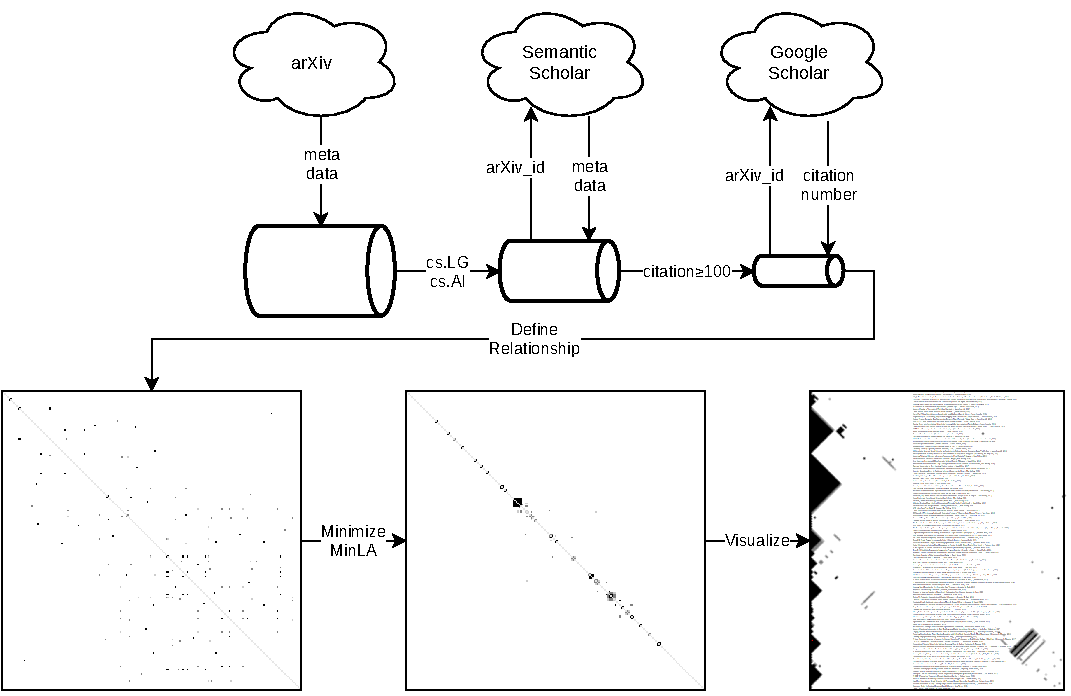
\includegraphics[width=0.8\textwidth]{images/fig1_long.pdf}
  \caption{The data processing pipeline.}
  \label{fig:1}
\end{figure}

\begin{abstract}
Deep Learning field is exploding.
We explore the relationship in authors of the highly cited arXiv papers from cs.LG and cs.AI categories.
We reorder the relationship matrix into proximate block diagonal form by minimize the minimum linear arrangement (MinLA) cost function using a simple parallel hill climbing algorithm.
We visualize the results as a fancy list of papers.
We hope this analysis can capture some structures of the Deep Learning community.


\end{abstract}


% keywords can be removed
\keywords{Information visualization \and Matrix reordering \and Minimum linear arrangement \and Block diagonal form \and Hill Climbing \and GPU}

% \section{Todo}
% The problem:

I am trying to find the field and terminology.
It is related to Matrix Reordering Methods. \cite{behrisch_matrix_2016}

This problem is equivalent to the \emph{minimum linear arrangement problem} (MinLA). \cite{goos_multi-scale_2002}
MinLA is introduced back in 1973 as the \emph{optimal linear ordering problem}. \cite{adolphson_optimal_1973}

It is a special case of \emph{quadratic assignment problem}, where every node is in a line and have equal unit distance to it's neighbors.

It is NP-complete. \cite{garey_simplified_1976}

\cite{goos_multi-scale_2002} provide a exact algorithm that can serve as the ground truth, which is better than naive enumerate $O(n!)$.

\cite{andrade_minimum_2017} provide an exact linear programming method, which can solve toy problems with only 10 nodes.

\cite{pantrigo_scatter_2012} uses evolutionary approach to solve a unweighted version of this problem. they call it the cutwidth minimization problem.

\cite{petit_experiments_2004} has thoroughly introduced lower bound methods and heristic methods, including the hill climbing method. which is good.
however, after that paper, evolutionary algorithms have been developed.
we re-engineer the hill climbing a bit, to make it faster.
we also try other methods like parallel hill climbing, to show it is possible to apply full flame evolutionary algorithm.

a Master thesis describe a GA approach of evolving better initial state for the hill climber optimization.

Preprocessing:

We can first detect the largest connected component, because if the graph is not connected, the sub-graphs can be solved independently.

Future direction:

push 1D (2D matrix reordering) to 2D (4D tensor reordering), maybe we can get a 2D visualization!


\section{Introduction}

Deep Learning as a field is exploding.
The number of papers is growing rapidly.

Luckily, arXiv acts as a central hub for important papers and opens to everyone.
This provides a chance for us to analyze those papers procedually.

We harvest the meta data from arXiv service.
And obtain the citation numbers from Semantic Scholar and Google Scholar.
We will see, although the total number of papers is big, the number of highly cited papers is relatively small.

We compare the authorships of the highly cited papers pairwisely to obtain a pairwise relationship matrix.
We reorder the relationship matrix by minimize the minimum linear arrangement (MinLA) cost function, so that the nodes that have relationship are arranged closer.
The optimization is done through a GPU augmented parallel hill climbing algorithm.
We observe that clusters are formed, indicating the structure of the research community.

Finally, we visualize the results as a sorted list of papers, with a corresponding image to indicate the community structure.
We will highlight several famous clusters.



\section{Data}
\subsection{Retrival}

arXiv is the largest hub for open access scientific papers.
It also supports the Open Archives Initiative (OAI),
so a large volume of metadata can be easily downloaded through the OAI interface.
\footnote{More about arXiv OAI: \url{https://arxiv.org/help/oa}}

In April 2021, we downloaded the metadata of 227,842 papers.
The analysis we have done is based on these metadata.
Our main interest field is Deep Learning.
Due to the computational resource constraints, we only processed two arXiv subcategories: cs.LG (Machine Learning) and cs.AI (Artificial Intelligence).
There are 93,911 papers in these two subcategories.

We filter the papers by the citation number.
The citation number of a paper is a commonly-used indicator.
However, arXiv metadata does not include any information about citations,
and accurate citation numbers are hard to obtain,
so we get the citation numbers from two third-party websites.

The first data source is Semantic Scholar (S2).
S2 provides additional metadata including the citation numbers of the scientific papers.
\footnote{More about Semantic Scholar API: \url{https://api.semanticscholar.org/}}
We can see from Fig. \ref{fig:s2_dist}, the citation number follows a power-law distribution, which means there are a few highly cited papers and many papers with much less citations.
Among them, 27,317 papers in 93,911 (roughly 29\%) have a citation number of zero.
Also we can notice from the figure that there is a hard cut-off at $10^4$, which might due to their system limitation.

\begin{figure}
    \centering
    \begin{minipage}{0.48\textwidth}
        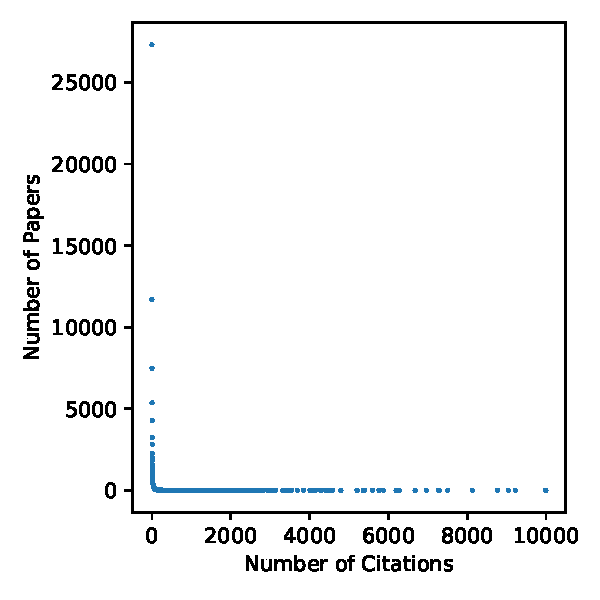
\includegraphics[width=\textwidth]{images/s2_dist.pdf}
    \end{minipage}%
    \begin{minipage}{0.48\textwidth}
        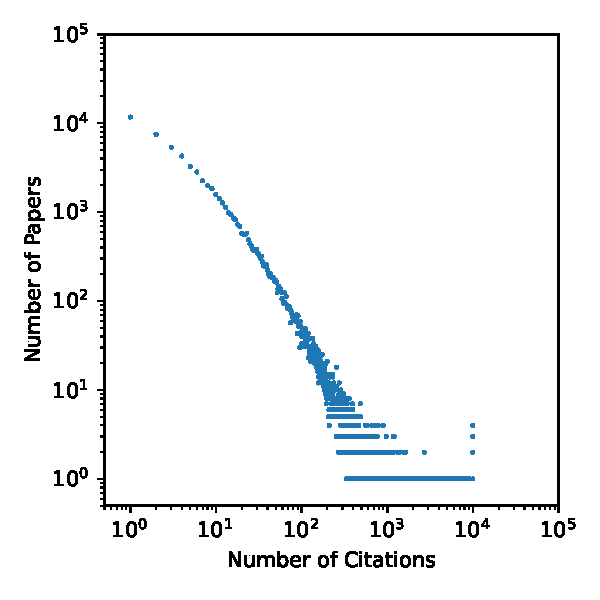
\includegraphics[width=\textwidth]{images/s2_dist_log.pdf}
    \end{minipage}
    \caption{Citation number follows a power-law distribution according to S2.
    (Left): Normal scale. (Right): Log-log scale excluding the zero-cited papers.
    Each dot represents \emph{a set of papers} with the same citation number, e.g. the first dot on the left plot represents all papers with 0 citation, and there are 27,317 of them.
    }
    \label{fig:s2_dist}
\end{figure}

We use the S2 citation numbers to filter out highly citated papers.
We keep 4,422 papers with S2 citation numbers larger than or equal to 100 as the highly cited papers.

The second data source is Google Scholar.
Google Scholar also provides citation numbers on its website.
However, it does not support API retrival due to unspecified reasons.
Getting citation numbers from Google Scholar can only be done semi-automatically.

The use of two data sources has both strengths and limitations,
so we ensemble two parts together by taking the mean of the two.
Fig. \ref{fig:distribution} shows the distribution of the highly cited papers.
\footnote{Raw metadata of the 4,422 papers can be downloaded at: \url{http://star-lab.ai/arxiv/arxiv_4422.tar.gz}}

\begin{figure}
    \centering
    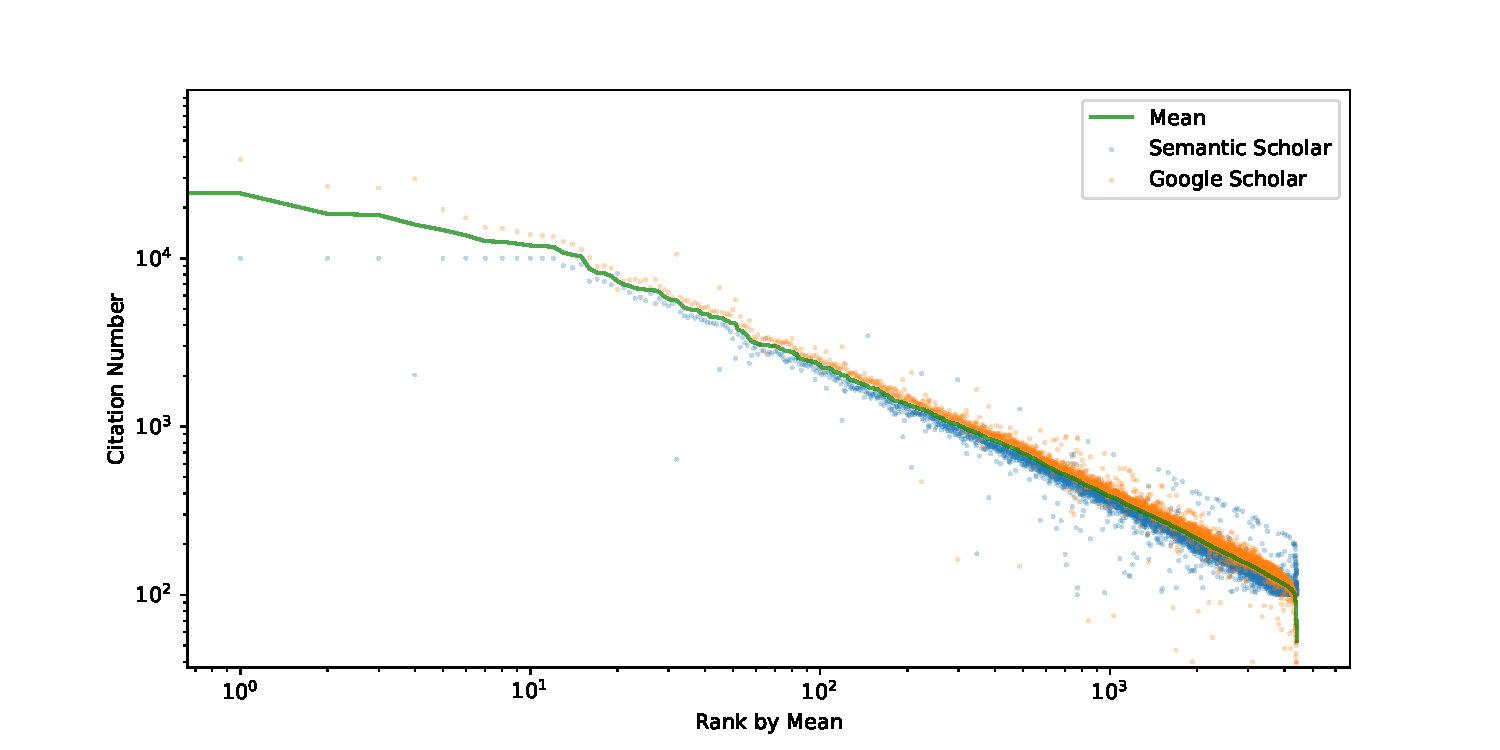
\includegraphics[width=\textwidth]{images/citation_number_distribution.pdf}
    \caption{Citation number distribution for highly cited 4,422 arXiv cs.LG and cs.AI papers.
        The blue dots are the Semantic Scholar citation numbers ($S2$),
        and the orange dots are the Google Scholar citation numbers ($GS$).
        For most of the papers, $GS$ are higher than $S2$.
        $S2$ are bounded by $10^4$, which might due to their system limitation.
        But $GS$ misses some papers which $S2$ consider them as highly cited.
        The green line is the mean of $S2$ and $GS$.
        Each dot represents the citation number of \emph{one} paper, 
        e.g. the first orange dot represents the citation number (69,774) reported by Google Scholar for the most highly cited paper (Rank 1).
    }
    \label{fig:distribution}
\end{figure}

\subsection{Relationship Between Papers}

Now we have 4,422 highly cited papers.
We define a undirected weighted network $G(V,E)$, with its nodes set $V$ to be the set of those papers, and its edges set $E$ to be the set of the relationships between papers.

Our objective is to reveal the structure of the research community.
Based on this objective, we define the weights $w_{i,j}$ of the edge between papers based on the overlaps in authorships.
We divide the authors of a paper into two classes: ($A$) the first author and the last author, ($B$) other authors which are neither the first nor the last author.

There are multiple inconsistencies in arXiv metadata and Semantic Scholar metadata, we tried to correct some errors, but still there are remaining ones.
In this case, we use the metadata from arXiv.

Class ($A$) always at least contains one author, and class ($B$) could be empty if there are no other authors.
We give a weight of 1.0 if class ($A$) of two papers overlap.
Otherwise, we give a weight of 0.5 if class ($A$) of one paper overlaps with ($B$) of another paper.
Otherwise, we give a weight of 0.3 if class ($B$) of two papers overlap.

This is an ad hoc method to define the relationships.
One can come up with other definitions and the pipeline will still work.

Fig. \ref{fig:matrix_random_arrangement} shows the adjacent matrix of the constructed network $G$ with a random arrangement (which is almost blank).

\begin{figure}
    \centering
    
\includegraphics[width=\textwidth]{images/random_arrangement.png}
    \caption{The relationship matrix in a random arrangement before matrix reordering.
        Dark grids mean they have values, which represent the author relationships between two papers.
        The diagonal line is defined to be 1.0.
        However, a 4422x4422 matrix with a random arrangement is almost meaningless to a human observer.
        (The image looks almost blank due to the sparsity of the matrix.)
    }
    \label{fig:matrix_random_arrangement}
\end{figure}


\section{Matrix Reordering}
In order to reveal the structure of the network $G$, we choose to reorder the matrix.
There are many ways to rearrange a symmetric matrix, Behrisch et al. \cite{behrisch_matrix_2016} provides a good review of those methods.
In practice, we notice that many methods will introduce so called the \emph{Off-diagonal Block Pattern} even when there is no such pattern in the data.
We consider this as an artifact of the algorithms.

We want to reorder the matrix into an proximate block diagonal form, so that all the papers produced by the same group will be arranged close to each other.
We achieve this by minimizing the weighted linear arrangement (LA) cost function:

\begin{equation}
    LA(G, \pi) = \sum_{ij \in E} w_{i,j} \cdot |\pi(i) - \pi(j)|
\end{equation}

where $\pi$ is a one-to-one function $V \rightarrow \{1,2,\cdots,|V|\}$ representing the permutation of the nodes in 1D, a.k.a the arrangement of the matrix;
$w_{i,j}$ is the weights of the edge between node $i$ and $j$.

In this paper, we use a normalized version of MinLA:
\begin{equation}
    LA(G, \pi) = \sum_{ij \in E} w_{i,j} \cdot \frac{|\pi(i) - \pi(j)|}{|V|^2}
\end{equation}

where $|V|$ is the number of nodes.

This is known as the minimum linear arrangement (MinLA) problem.
The MinLA problem was introduced in 1973 as the \emph{optimal linear ordering problem} \cite{adolphson_optimal_1973}.
It is a special case of the \emph{quadratic assignment problem}, where every node is in a line and have equal unit distance to it's neighbors.
It is proved to be a NP-complete problem \cite{garey_simplified_1976},
One should not expect to solve a large scale NP-complete using exact methods, 
e.g. \cite{andrade_minimum_2017} only works with no more than 20 nodes.
Petit \cite{petit_experiments_2004} has thoroughly introduced some heristic methods that can provide approximate optimal solutions to the MinLA problem, 
including the hill climbing method.

Basic hill climbing algorithm can be described in Algo. \ref{algo:hillclimbing}. 

\begin{algorithm}
    \caption{Hill Climbing}\label{algo:hillclimbing}
    \begin{algorithmic}[1]
        \State \textbf{while} not Terminated:
        \State \hskip2em $i,j \leftarrow \textbf{random}()$
        \State \hskip2em \textbf{if} \textbf{swapCanReduceLA}(i,j): \Comment{This can be done in $O(|V|)$.}
        \State \hskip4em \textbf{swap}(i,j)
    \end{algorithmic}
\end{algorithm}

To take advantage of the power of parallel computing, we propose a GPU augmented hill climbing method, described in Algo. \ref{algo:gpu_hill_climbing}.

\begin{algorithm}
    \caption{GPU augmented Hill Climbing}\label{algo:gpu_hill_climbing}
    \begin{algorithmic}[1]
        \State \textbf{while} not Terminated:
        \State \hskip2em Detect pairs which if swapped will reduce the LA cost \Comment{With 32,768 threads on GPU}
        \State \hskip2em Sort pairs by the gains (the amount that can be reduced)
        \State \hskip2em Remove conflicted pairs with less gains
        \State \hskip2em Swap all pairs remained
        \State \hskip2em If number of the found pairs is small:
        \State \hskip4em Double the number of parallel threads for detection until limit hit
    \end{algorithmic}
\end{algorithm}

Fig. \ref{fig:gpu_hill_climbing} shows the comparison of Algo. \ref{algo:hillclimbing} and \ref{algo:gpu_hill_climbing} in wall time.

\begin{figure}
    \centering
    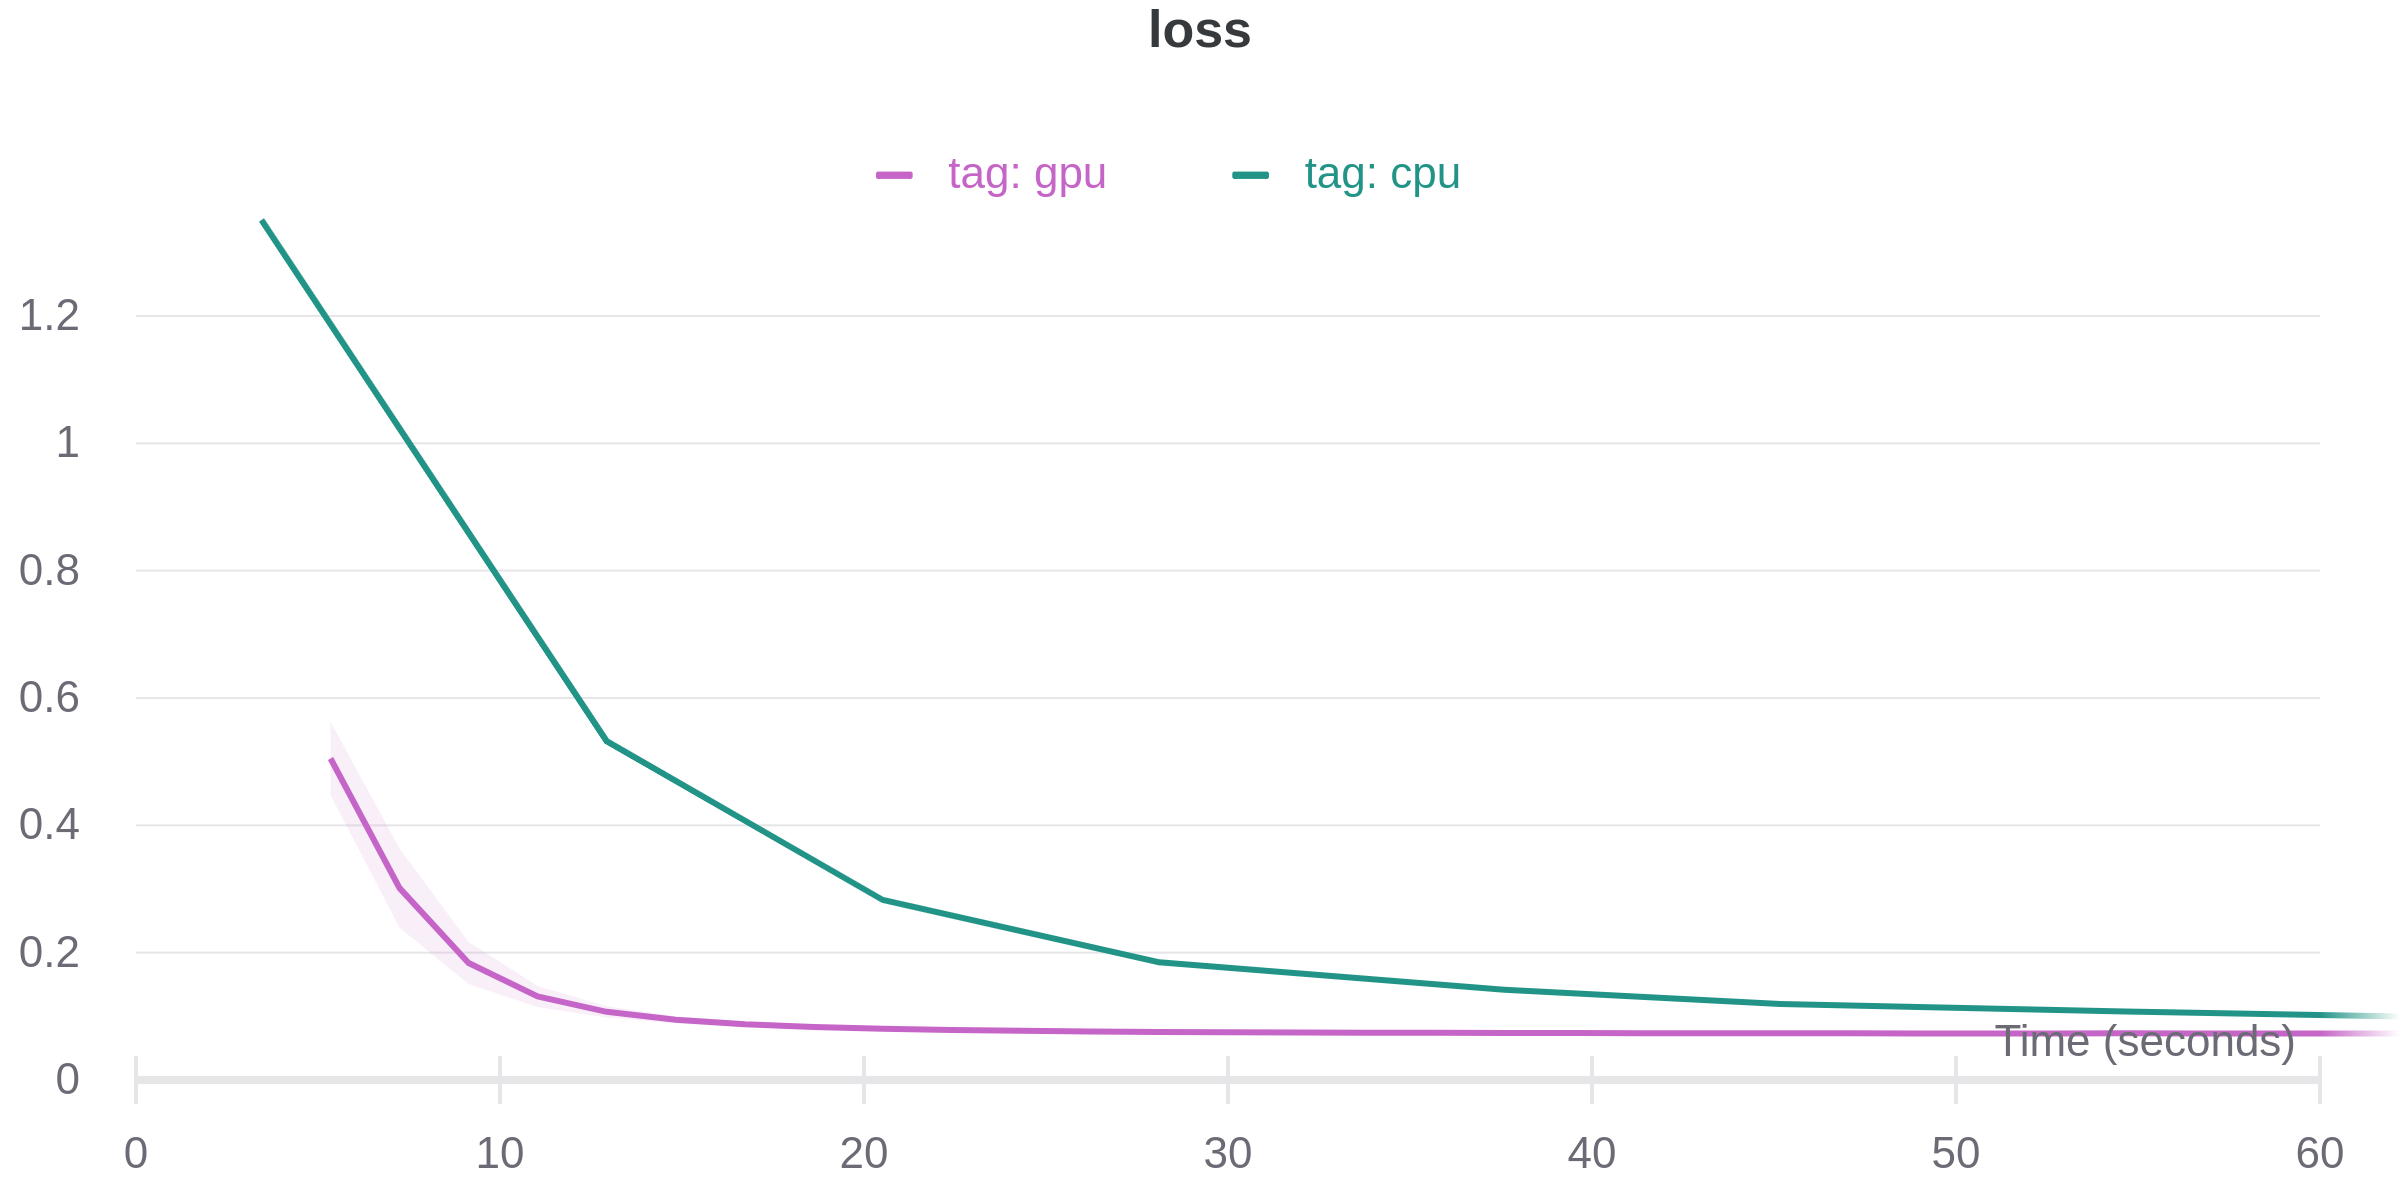
\includegraphics[width=0.8\textwidth]{images/curve_60s.png}
    \caption{A comparison of the first 60 seconds of the optimization curve of Algo. \ref{algo:hillclimbing} and \ref{algo:gpu_hill_climbing}. 
    Averaged over 100 independent runs.
    The GPU augmented algorithm is better than the basic algorithm in wall time.
    }
    \label{fig:gpu_hill_climbing}
\end{figure}

Both the basic hill climbing algorithm and the GPU augmented hill climbing algorithm are implemented in Python and accelerated by Numba \cite{lam_numba_2015}.
One instance of Algo. \ref{algo:hillclimbing} uses one Intel 6230 CPU core.
One instance of Algo. \ref{algo:gpu_hill_climbing} uses one Intel 6130 CPU core and one NVIDIA Tesla V100s GPU.

Both methods are fast enough to get reasonable good results in less than one minute, though the GPU augmented version can achieve better solutions in general.
One of the results can be visualized in Fig. \ref{fig:optimization_results}.

\begin{figure}
    \centering
    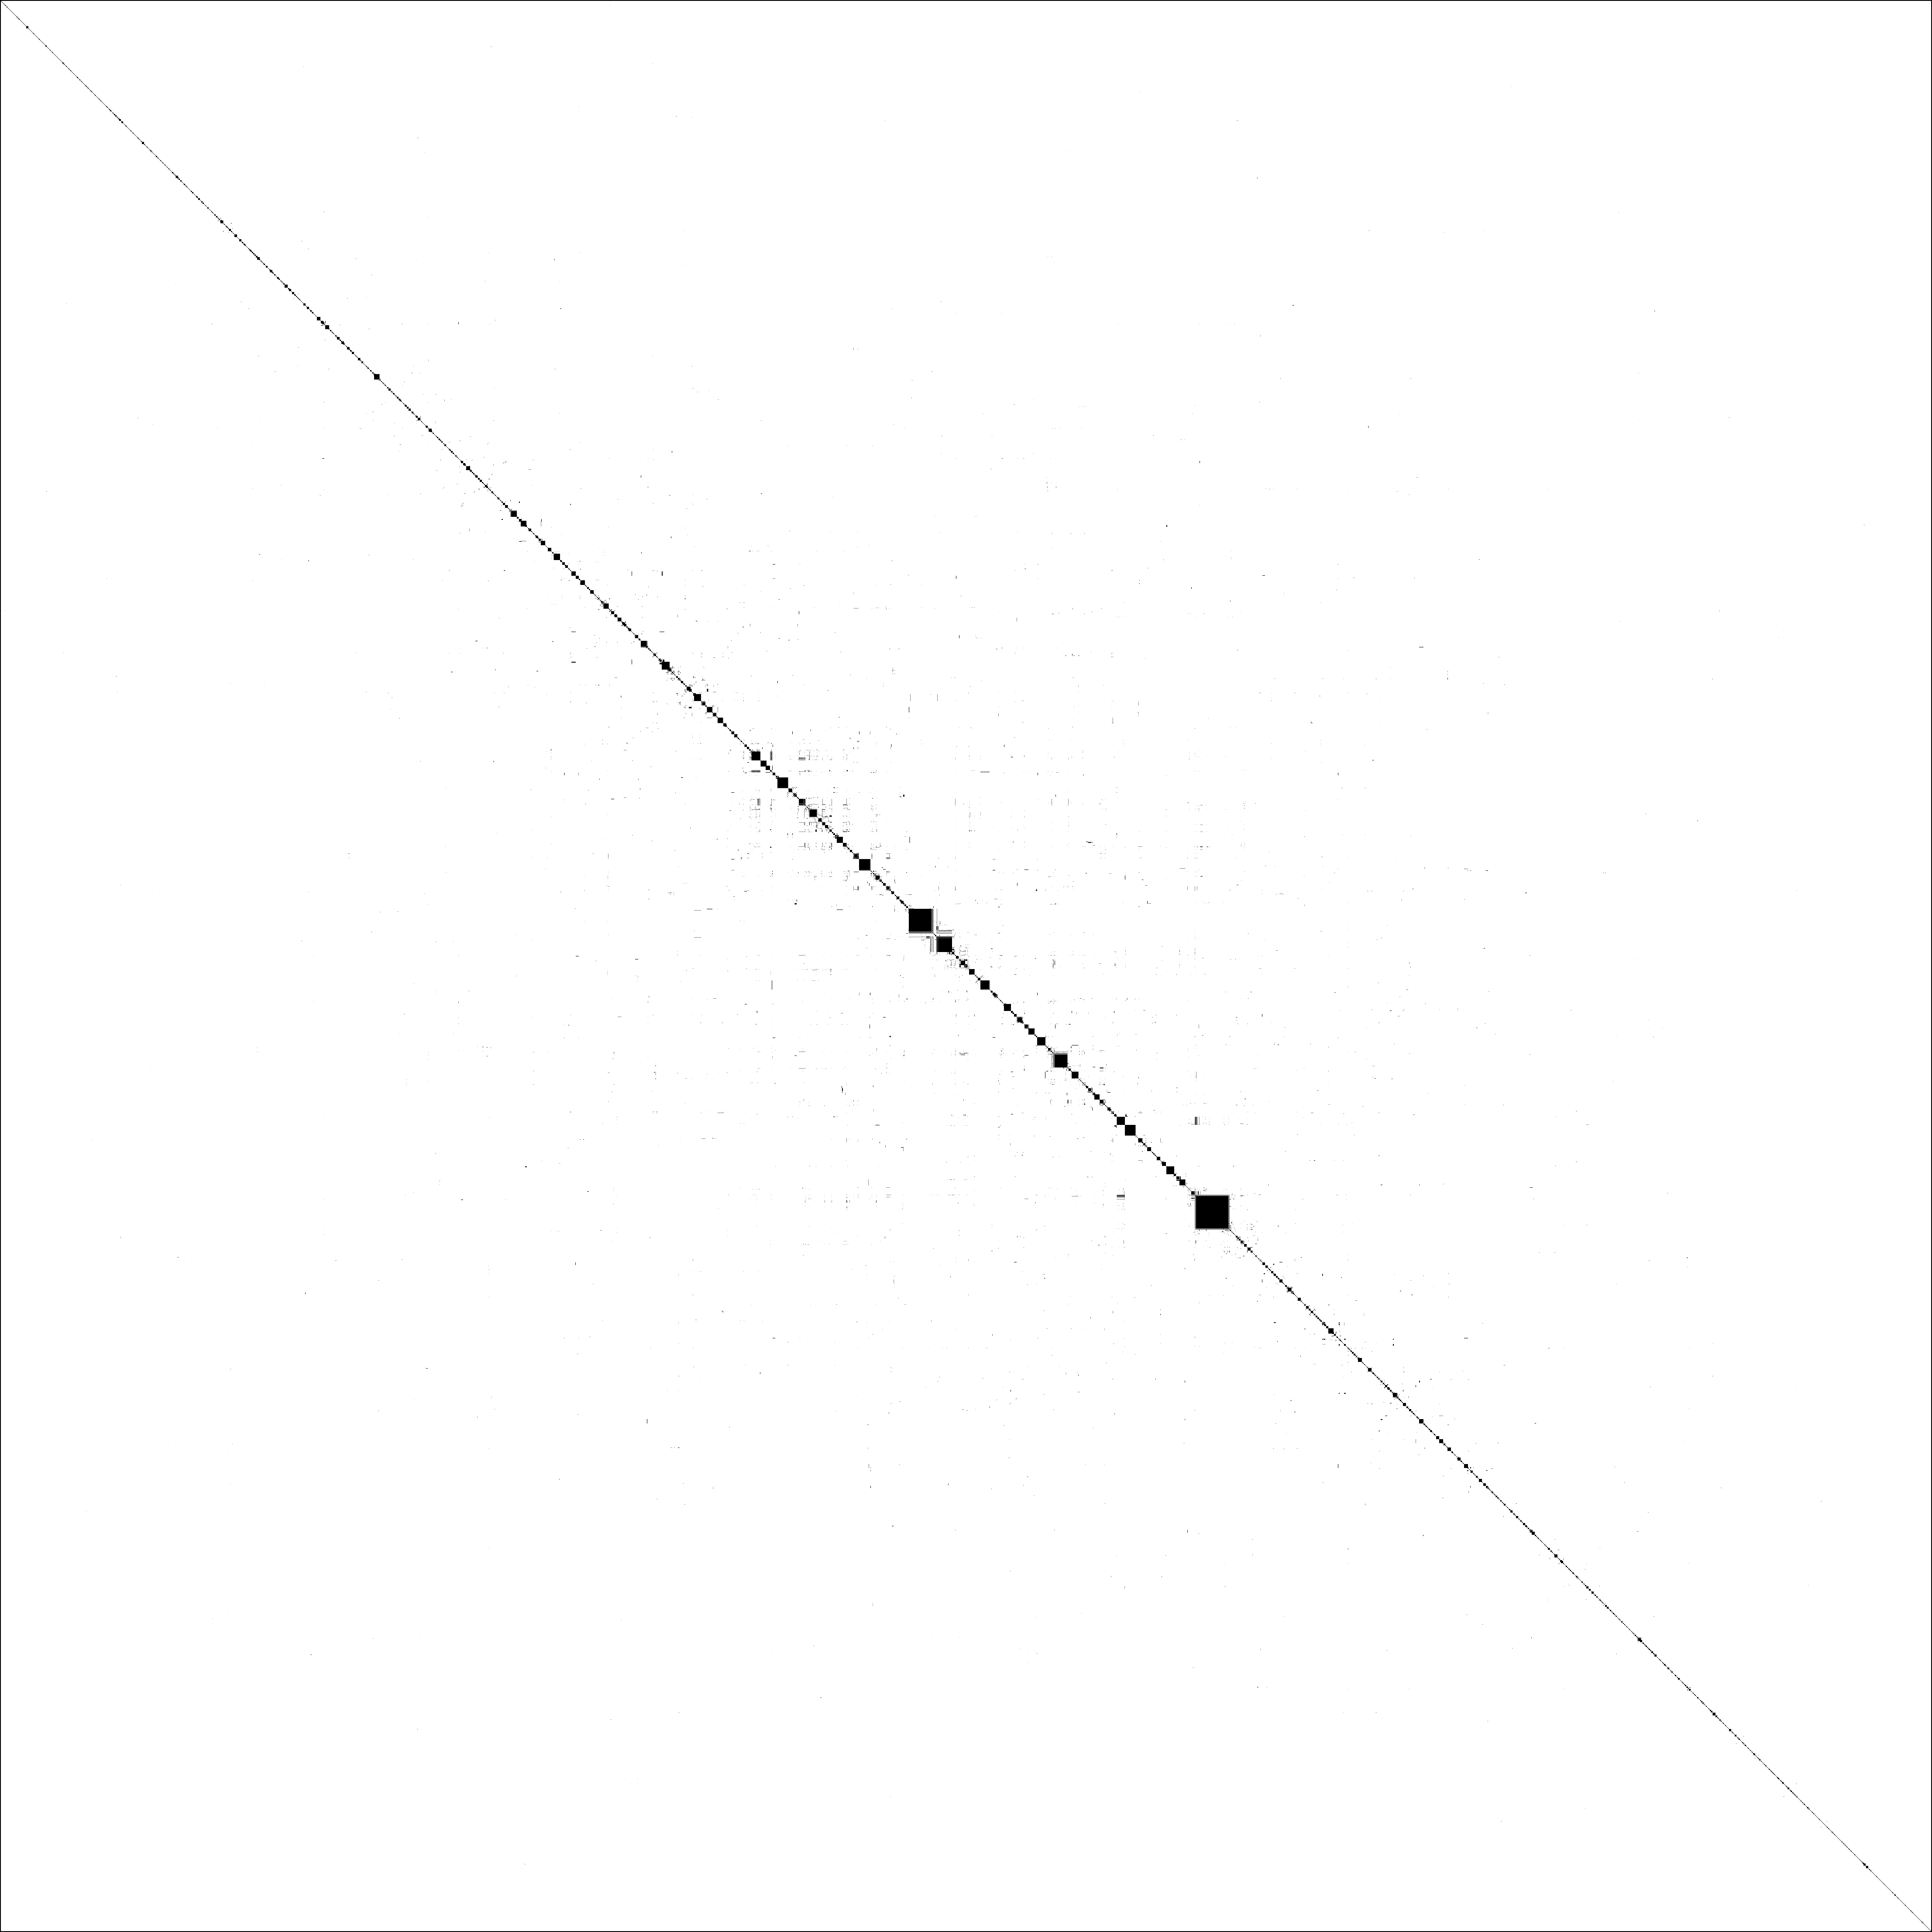
\includegraphics[width=\textwidth]{images/seed_94_step_0181.png}
    \caption{The most optimal solution of Algo. \ref{algo:gpu_hill_climbing} in 100 runs, with LA=0.06596.
    Computing this solution takes about 4 minutes.
    Now we can easily observe the structure of the research community.
    The largest square in the center represents the papers related to Yoshua Bengio;
    the second and third squares close to each other represents the papers related to Sergey Levine and Pieter Abbeel.
    Other clusters can be observed.
    }
    \label{fig:optimization_results}
\end{figure}

However, it still slightly suffers from local optima.
In order to get more optimal results, one can not rely on running the algorithm for longer.

Our best results are achieved by searching with 100 independent runs with random initialization.
However, we observe that the initial states matter more than trying different choices during optimization.
Thus, an evolutionary approach \cite{eppley2001} searching for better initial states might be better than our random initialization.


\section{Visualization}
We design a way to visually present the final arranged results.
The goal is to easily navigate through with useful visual clues.
The final visualization is made as a web page.
\footnote{The final visualization can be accessed at: \url{http://star-lab.ai/arxiv/}}

On the left, the vertical line is made of the diagonal line of the relationship matrix.
The larger the clusters are, the more collaberations are there in those groups.

On the right, they are the reordered list of all papers.
One can easily search keywords to locate interesting parts of the list.


\section{Discussion}
In this paper, we define relationships between papers by the overlap in authors.
Future work can explore different relationships, e.g. the interactions of the authors' Twitter accounts, or the similarity in the abstract, etc.

The implementation can be further optimized by using sparse matrix presentation instead of a 2D array.


\section{Conclusion}
In this paper, we presented a pipeline to process metadata of highly cited arXiv papers in two subcategories: cs.LG and cs.AI.
Those metadata comes from different sources.
We built a relationship matrix by defining the relationships in authorships.
We reordered the matrix by optimizing the LA loss function using a GPU augmented hill climbing method.
The results of the optimization reveal the structure of the research community.
We presented the final results as a web page to help other researchers to understand this social structure better.


\section{Acknowledge}
Computations were performed on the Vermont Advanced Computing Core supported in part by NSF award No. OAC-1827314.

\bibliographystyle{unsrt}  
\bibliography{references}  %%% Remove comment to use the external .bib file (using bibtex).

\end{document}
